\documentclass{standalone}
\usepackage{tikz}
\begin{document}
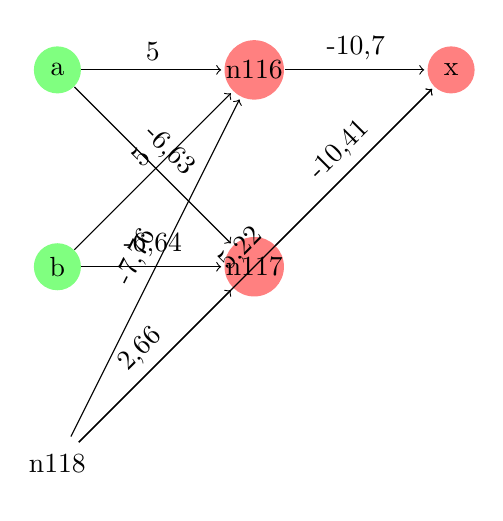
\begin{tikzpicture}[shorten >=1pt,->,draw=black!,node distance=2.5cm]
\tikzstyle{neuron}=[circle,fill=black!25,minimum size=17pt,inner sep=0pt]
\tikzstyle{constant}=[neuron, fill=white!50];
\tikzstyle{sigmoid}=[neuron, fill=red!50];
\tikzstyle{identity}=[neuron, fill=green!50];
\node [identity] (a) {a};
\node [identity,below of=a] (b) {b};
\node [constant,below of=b] (n118) {n118};
\node [sigmoid,right of=a] (n116) {n116};
\node [sigmoid,below of=n116] (n117) {n117};
\node [sigmoid,right of=n116] (x) {x};
\path[every node/.style={sloped,anchor=south,auto=false}]
(n118) edge node {5,22} (x)
(n118) edge node {-7,76} (n116)
(n118) edge node {2,66} (n117)
(n116) edge node {-10,7} (x)
(n117) edge node {-10,41} (x)
(a) edge node {-6,63} (n117)
(a) edge node {5} (n116)
(b) edge node {5} (n116)
(b) edge node {-6,64} (n117)
;\end{tikzpicture}
\end{document}